% Created by tikzDevice version 0.12 on 2018-09-28 04:16:26
% !TEX encoding = UTF-8 Unicode
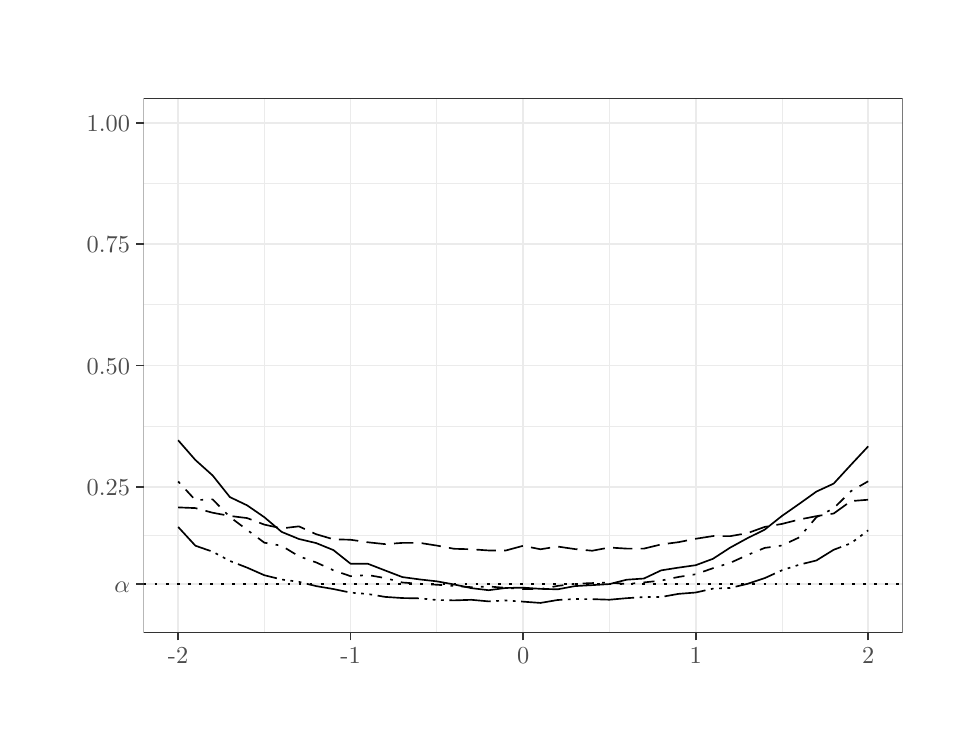
\begin{tikzpicture}[x=1pt,y=1pt]
\definecolor{fillColor}{RGB}{255,255,255}
\path[use as bounding box,fill=fillColor,fill opacity=0.00] (0,0) rectangle (325.21,252.94);
\begin{scope}
\path[clip] (  0.00,  0.00) rectangle (325.21,252.94);
\definecolor{drawColor}{RGB}{255,255,255}
\definecolor{fillColor}{RGB}{255,255,255}

\path[draw=drawColor,line width= 0.6pt,line join=round,line cap=round,fill=fillColor] (  0.00,  0.00) rectangle (325.21,252.94);
\end{scope}
\begin{scope}
\path[clip] ( 41.90, 34.26) rectangle (316.18,227.38);
\definecolor{fillColor}{RGB}{255,255,255}

\path[fill=fillColor] ( 41.90, 34.26) rectangle (316.18,227.38);
\definecolor{drawColor}{gray}{0.92}

\path[draw=drawColor,line width= 0.3pt,line join=round] ( 41.90, 69.37) --
	(316.18, 69.37);

\path[draw=drawColor,line width= 0.3pt,line join=round] ( 41.90,108.87) --
	(316.18,108.87);

\path[draw=drawColor,line width= 0.3pt,line join=round] ( 41.90,152.76) --
	(316.18,152.76);

\path[draw=drawColor,line width= 0.3pt,line join=round] ( 41.90,196.65) --
	(316.18,196.65);

\path[draw=drawColor,line width= 0.3pt,line join=round] ( 85.53, 34.26) --
	( 85.53,227.38);

\path[draw=drawColor,line width= 0.3pt,line join=round] (147.87, 34.26) --
	(147.87,227.38);

\path[draw=drawColor,line width= 0.3pt,line join=round] (210.21, 34.26) --
	(210.21,227.38);

\path[draw=drawColor,line width= 0.3pt,line join=round] (272.55, 34.26) --
	(272.55,227.38);

\path[draw=drawColor,line width= 0.6pt,line join=round] ( 41.90, 51.81) --
	(316.18, 51.81);

\path[draw=drawColor,line width= 0.6pt,line join=round] ( 41.90, 86.93) --
	(316.18, 86.93);

\path[draw=drawColor,line width= 0.6pt,line join=round] ( 41.90,130.82) --
	(316.18,130.82);

\path[draw=drawColor,line width= 0.6pt,line join=round] ( 41.90,174.71) --
	(316.18,174.71);

\path[draw=drawColor,line width= 0.6pt,line join=round] ( 41.90,218.60) --
	(316.18,218.60);

\path[draw=drawColor,line width= 0.6pt,line join=round] ( 54.37, 34.26) --
	( 54.37,227.38);

\path[draw=drawColor,line width= 0.6pt,line join=round] (116.70, 34.26) --
	(116.70,227.38);

\path[draw=drawColor,line width= 0.6pt,line join=round] (179.04, 34.26) --
	(179.04,227.38);

\path[draw=drawColor,line width= 0.6pt,line join=round] (241.38, 34.26) --
	(241.38,227.38);

\path[draw=drawColor,line width= 0.6pt,line join=round] (303.71, 34.26) --
	(303.71,227.38);
\definecolor{drawColor}{RGB}{0,0,0}

\path[draw=drawColor,line width= 0.6pt,dash pattern=on 1pt off 3pt on 4pt off 3pt ,line join=round] ( 54.37, 88.96) --
	( 60.60, 82.22) --
	( 66.83, 82.50) --
	( 73.07, 76.11) --
	( 79.30, 71.48) --
	( 85.53, 66.84) --
	( 91.77, 65.72) --
	( 98.00, 61.93) --
	(104.24, 59.71) --
	(110.47, 56.87) --
	(116.70, 54.73) --
	(122.94, 55.15) --
	(129.17, 54.06) --
	(135.40, 52.45) --
	(141.64, 51.99) --
	(147.87, 51.64) --
	(154.10, 51.22) --
	(160.34, 50.76) --
	(166.57, 51.01) --
	(172.81, 50.52) --
	(179.04, 50.09) --
	(185.27, 50.06) --
	(191.51, 51.22) --
	(197.74, 51.99) --
	(203.97, 52.24) --
	(210.21, 52.45) --
	(216.44, 51.88) --
	(222.68, 52.48) --
	(228.91, 53.15) --
	(235.14, 54.45) --
	(241.38, 55.43) --
	(247.61, 57.61) --
	(253.84, 59.54) --
	(260.08, 62.38) --
	(266.31, 64.95) --
	(272.55, 65.82) --
	(278.78, 68.74) --
	(285.01, 76.04) --
	(291.25, 79.24) --
	(297.48, 85.45) --
	(303.71, 89.03);

\path[draw=drawColor,line width= 0.6pt,dash pattern=on 15pt off 2pt on 1pt off 2pt on 1pt off 2pt on 1pt off 2pt ,line join=round] ( 54.37, 72.53) --
	( 60.60, 65.75) --
	( 66.83, 63.58) --
	( 73.07, 60.24) --
	( 79.30, 57.82) --
	( 85.53, 55.08) --
	( 91.77, 53.54) --
	( 98.00, 52.69) --
	(104.24, 51.15) --
	(110.47, 50.09) --
	(116.70, 48.79) --
	(122.94, 48.30) --
	(129.17, 47.25) --
	(135.40, 46.83) --
	(141.64, 46.72) --
	(147.87, 46.13) --
	(154.10, 45.99) --
	(160.34, 46.20) --
	(166.57, 45.63) --
	(172.81, 45.95) --
	(179.04, 45.53) --
	(185.27, 45.07) --
	(191.51, 46.13) --
	(197.74, 46.48) --
	(203.97, 46.44) --
	(210.21, 46.23) --
	(216.44, 46.79) --
	(222.68, 47.18) --
	(228.91, 47.21) --
	(235.14, 48.34) --
	(241.38, 48.83) --
	(247.61, 50.23) --
	(253.84, 50.48) --
	(260.08, 51.96) --
	(266.31, 54.03) --
	(272.55, 56.87) --
	(278.78, 58.87) --
	(285.01, 60.42) --
	(291.25, 64.28) --
	(297.48, 66.63) --
	(303.71, 71.30);

\path[draw=drawColor,line width= 0.6pt,dash pattern=on 7pt off 3pt ,line join=round] ( 54.37, 79.59) --
	( 60.60, 79.34) --
	( 66.83, 77.66) --
	( 73.07, 76.50) --
	( 79.30, 75.73) --
	( 85.53, 73.37) --
	( 91.77, 72.00) --
	( 98.00, 72.74) --
	(104.24, 69.90) --
	(110.47, 68.07) --
	(116.70, 67.90) --
	(122.94, 66.98) --
	(129.17, 66.32) --
	(135.40, 66.77) --
	(141.64, 66.77) --
	(147.87, 65.79) --
	(154.10, 64.63) --
	(160.34, 64.46) --
	(166.57, 64.03) --
	(172.81, 64.03) --
	(179.04, 65.72) --
	(185.27, 64.46) --
	(191.51, 65.44) --
	(197.74, 64.53) --
	(203.97, 63.93) --
	(210.21, 65.09) --
	(216.44, 64.70) --
	(222.68, 64.70) --
	(228.91, 66.21) --
	(235.14, 67.02) --
	(241.38, 68.25) --
	(247.61, 69.23) --
	(253.84, 69.20) --
	(260.08, 70.28) --
	(266.31, 72.53) --
	(272.55, 73.62) --
	(278.78, 75.20) --
	(285.01, 76.43) --
	(291.25, 77.38) --
	(297.48, 81.87) --
	(303.71, 82.36);

\path[draw=drawColor,line width= 0.6pt,line join=round] ( 54.37,103.85) --
	( 60.60, 96.72) --
	( 66.83, 91.14) --
	( 73.07, 83.31) --
	( 79.30, 80.33) --
	( 85.53, 76.04) --
	( 91.77, 70.74) --
	( 98.00, 68.18) --
	(104.24, 66.70) --
	(110.47, 64.17) --
	(116.70, 59.22) --
	(122.94, 59.22) --
	(129.17, 56.80) --
	(135.40, 54.41) --
	(141.64, 53.57) --
	(147.87, 52.87) --
	(154.10, 51.74) --
	(160.34, 50.41) --
	(166.57, 49.67) --
	(172.81, 50.48) --
	(179.04, 50.59) --
	(185.27, 50.16) --
	(191.51, 49.99) --
	(197.74, 51.15) --
	(203.97, 51.50) --
	(210.21, 51.88) --
	(216.44, 53.46) --
	(222.68, 53.89) --
	(228.91, 56.84) --
	(235.14, 57.82) --
	(241.38, 58.70) --
	(247.61, 61.01) --
	(253.84, 65.05) --
	(260.08, 68.46) --
	(266.31, 71.55) --
	(272.55, 76.50) --
	(278.78, 80.85) --
	(285.01, 85.31) --
	(291.25, 88.19) --
	(297.48, 94.97) --
	(303.71,101.64);

\path[draw=drawColor,line width= 0.6pt,dash pattern=on 1pt off 3pt ,line join=round] ( 41.90, 51.81) -- (316.18, 51.81);
\definecolor{drawColor}{gray}{0.20}

\path[draw=drawColor,line width= 0.6pt,line join=round,line cap=round] ( 41.90, 34.26) rectangle (316.18,227.38);
\end{scope}
\begin{scope}
\path[clip] (  0.00,  0.00) rectangle (325.21,252.94);
\definecolor{drawColor}{gray}{0.30}

\node[text=drawColor,anchor=base east,inner sep=0pt, outer sep=0pt, scale=  0.88] at ( 36.95, 48.78) {$\alpha$};

\node[text=drawColor,anchor=base east,inner sep=0pt, outer sep=0pt, scale=  0.88] at ( 36.95, 83.90) {$0.25$};

\node[text=drawColor,anchor=base east,inner sep=0pt, outer sep=0pt, scale=  0.88] at ( 36.95,127.79) {$0.50$};

\node[text=drawColor,anchor=base east,inner sep=0pt, outer sep=0pt, scale=  0.88] at ( 36.95,171.68) {$0.75$};

\node[text=drawColor,anchor=base east,inner sep=0pt, outer sep=0pt, scale=  0.88] at ( 36.95,215.57) {$1.00$};
\end{scope}
\begin{scope}
\path[clip] (  0.00,  0.00) rectangle (325.21,252.94);
\definecolor{drawColor}{gray}{0.20}

\path[draw=drawColor,line width= 0.6pt,line join=round] ( 39.15, 51.81) --
	( 41.90, 51.81);

\path[draw=drawColor,line width= 0.6pt,line join=round] ( 39.15, 86.93) --
	( 41.90, 86.93);

\path[draw=drawColor,line width= 0.6pt,line join=round] ( 39.15,130.82) --
	( 41.90,130.82);

\path[draw=drawColor,line width= 0.6pt,line join=round] ( 39.15,174.71) --
	( 41.90,174.71);

\path[draw=drawColor,line width= 0.6pt,line join=round] ( 39.15,218.60) --
	( 41.90,218.60);
\end{scope}
\begin{scope}
\path[clip] (  0.00,  0.00) rectangle (325.21,252.94);
\definecolor{drawColor}{gray}{0.20}

\path[draw=drawColor,line width= 0.6pt,line join=round] ( 54.37, 31.51) --
	( 54.37, 34.26);

\path[draw=drawColor,line width= 0.6pt,line join=round] (116.70, 31.51) --
	(116.70, 34.26);

\path[draw=drawColor,line width= 0.6pt,line join=round] (179.04, 31.51) --
	(179.04, 34.26);

\path[draw=drawColor,line width= 0.6pt,line join=round] (241.38, 31.51) --
	(241.38, 34.26);

\path[draw=drawColor,line width= 0.6pt,line join=round] (303.71, 31.51) --
	(303.71, 34.26);
\end{scope}
\begin{scope}
\path[clip] (  0.00,  0.00) rectangle (325.21,252.94);
\definecolor{drawColor}{gray}{0.30}

\node[text=drawColor,anchor=base,inner sep=0pt, outer sep=0pt, scale=  0.88] at ( 54.37, 23.25) {-2};

\node[text=drawColor,anchor=base,inner sep=0pt, outer sep=0pt, scale=  0.88] at (116.70, 23.25) {-1};

\node[text=drawColor,anchor=base,inner sep=0pt, outer sep=0pt, scale=  0.88] at (179.04, 23.25) {0};

\node[text=drawColor,anchor=base,inner sep=0pt, outer sep=0pt, scale=  0.88] at (241.38, 23.25) {1};

\node[text=drawColor,anchor=base,inner sep=0pt, outer sep=0pt, scale=  0.88] at (303.71, 23.25) {2};
\end{scope}
\end{tikzpicture}
